\documentclass{standalone}
% This file was created with tikzplotlib v0.9.15.

\usepackage{siunitx}
\usepackage{pgfplots}
% and optionally (as of Pgfplots 1.3):
\pgfplotsset{compat=newest}
\pgfplotsset{plot coordinates/math parser=false}
\newlength\figureheight
\newlength\figurewidth

\newcommand{\Set}[1]{\mathcal{#1}}
\newcommand{\Vector}[1]{\bm{\MakeLowercase{#1}}}
\newcommand{\Operator}[1]{\bm{\MakeUppercase{#1}}}
%%%%%%%%%%
\DeclareMathAlphabet{\mathsfbr}{OT1}{cmss}{m}{n}%for math sans serif (cmss)
\SetMathAlphabet{\mathsfbr}{bold}{OT1}{cmss}{bx}{n}%for math sans serif (cmss)
\DeclareRobustCommand{\msf}[1]{%
  \ifcat\noexpand#1\relax\msfgreek{#1}\else\mathsfbr{#1}\fi%for math sans serif (cmss)
}
\DeclareFontEncoding{LGR}{}{} % or load \usepackage{textgreek}
\DeclareSymbolFont{sfgreek}{LGR}{cmss}{m}{n}
\SetSymbolFont{sfgreek}{bold}{LGR}{cmss}{bx}{n}
\DeclareMathSymbol{\sXi}{\mathalpha}{sfgreek}{`X}
\DeclareMathSymbol{\sUpsilon}{\mathalpha}{sfgreek}{`U}

\begin{document}

% This file was created with tikzplotlib v0.9.15.
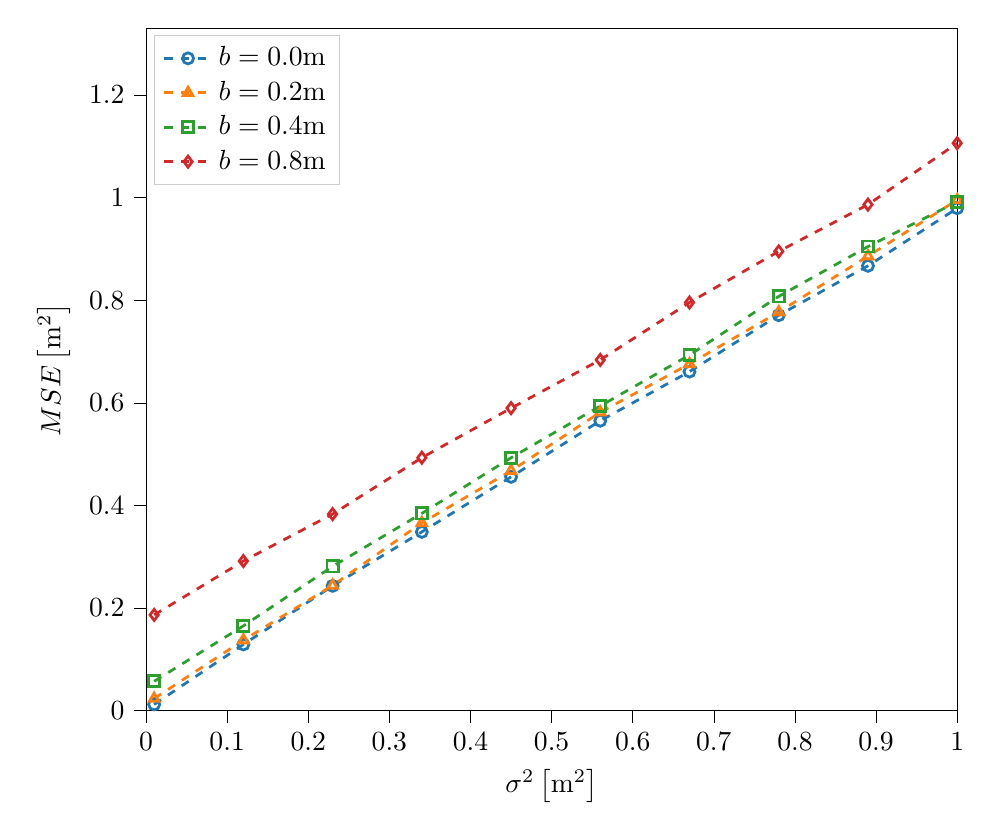
\begin{tikzpicture}

\definecolor{color0}{rgb}{0.12156862745098,0.466666666666667,0.705882352941177}
\definecolor{color1}{rgb}{1,0.498039215686275,0.0549019607843137}
\definecolor{color2}{rgb}{0.172549019607843,0.627450980392157,0.172549019607843}
\definecolor{color3}{rgb}{0.83921568627451,0.152941176470588,0.156862745098039}

\begin{axis}[
width=0.98\linewidth,
legend cell align={left},
legend style={
  fill opacity=0.8,
  draw opacity=1,
  text opacity=1,
  at={(0.01,0.99)},
  anchor=north west,
  draw=white!80!black
},
tick align=outside,
tick pos=left,
x grid style={white!69.0196078431373!black},
xlabel={$\sigma^2 \left[ \si{m^2} \right]$},
xmin=0, xmax=1,
xtick style={color=black},
y grid style={white!69.0196078431373!black},
ylabel={$MSE \left[ \si{m^2} \right]$},
ymin=0, ymax=1.33,
ytick style={color=black}
]
\addplot [dashed, semithick, color0, line width=1, mark=o, mark options={solid, color0}, mark repeat=1]
table {%
0.01 0.0122525
0.12 0.12904725
0.23 0.243276
0.34 0.34843125
0.45 0.4556785
0.56 0.56506525
0.67 0.660807
0.78 0.7707015
0.89 0.8669665
1 0.9791925
};
\addlegendentry{$b = 0.0 \si{m}$}
\addplot [dashed, semithick, color1, line width=1, mark=triangle, mark options={solid, color1}, mark repeat=1]
table {%
0.01 0.02359825
0.12 0.13738725
0.23 0.24410675
0.34 0.36601325
0.45 0.4674355
0.56 0.58160775
0.67 0.67580775
0.78 0.7767805
0.89 0.88588075
1 0.9952815
};
\addlegendentry{$b = 0.2 \si{m}$}
\addplot [dashed, semithick, color2, line width=1, mark=square, mark options={solid, color2}, mark repeat=1]
table {%
0.01 0.0573485
0.12 0.16528375
0.23 0.28123375
0.34 0.38452075
0.45 0.49292375
0.56 0.59386775
0.67 0.69310425
0.78 0.80736125
0.89 0.904471
1 0.99166275
};
\addlegendentry{$b = 0.4 \si{m}$}
\addplot [dashed, semithick, color3, line width=1, mark=diamond, mark options={solid, color3}, mark repeat=1]
table {%
0.01 0.1867005
0.12 0.29166775
0.23 0.3831255
0.34 0.49306925
0.45 0.58959275
0.56 0.683626
0.67 0.79554575
0.78 0.895135
0.89 0.98625425
1 1.10590225
};
\addlegendentry{$b = 0.8 \si{m}$}
\end{axis}

\end{tikzpicture}

\end{document}